\documentclass{standalone}
\usepackage{tikz}
\usepackage{ctex,siunitx}
\setCJKmainfont{Noto Serif CJK SC}
\usepackage{tkz-euclide}
\usepackage{amsmath}
\usetikzlibrary{patterns, calc}
\usetikzlibrary {decorations.pathmorphing, decorations.pathreplacing, decorations.shapes,}
\begin{document}
\small
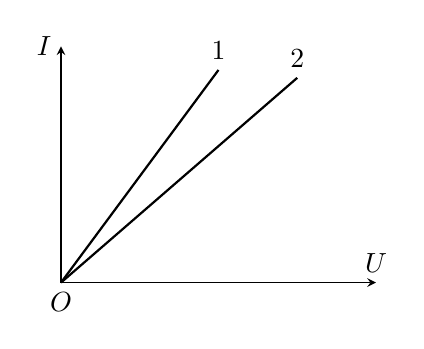
\begin{tikzpicture}[>=stealth]
  \draw[thin,<->] (0,3)node [left]{$I$}--(0,0)node [below]{$O$}--(4,0)node [above]{$U$};
  \draw[thick] (0,0)--(2,2.7)node [above]{1};
  \draw[thick] (0,0)--(3,2.6) node [above]{2};
\end{tikzpicture}
\end{document}